% ==== Document Class & Packages =====
\documentclass[12pt,hidelinks]{article}
	\usepackage[explicit]{titlesec}
	\usepackage{titletoc}
	\usepackage{tocloft}
	\usepackage{charter}
	\usepackage[many]{tcolorbox}
	\usepackage{amsmath}
	\usepackage{graphicx}
	\usepackage{xcolor}
	\usepackage{tikz,lipsum,lmodern}
	\usetikzlibrary{calc}
	\usepackage[english]{babel}
	\usepackage{fancyhdr}
	\usepackage{mathrsfs}
	\usepackage{empheq}
	\usepackage{fourier}% change to lmodern if fourier is no available
	\usepackage{wrapfig}
	\usepackage{fancyref}
	\usepackage{hyperref}
	\usepackage{cleveref}
	\usepackage{listings}
	\usepackage{varwidth}
	\usepackage{longfbox}
	\usepackage{geometry}
	\usepackage{marginnote}
	\tcbuselibrary{theorems}
	\tcbuselibrary{breakable, skins}
	\tcbuselibrary{listings, documentation}
	\geometry{
		letterpaper,
		left=33mm,
		right=33mm,
		top=20mm}
% ========= Path to images ============
%   - Direct the computer on the path 
% 	  to the folder containg the images
% =====================================
\graphicspath{{./images/}}
% ============= Macros ================
\newcommand{\fillin}{\underline{\hspace{.75in}}{\;}}
\newcommand{\solution}{\textcolor{mordantred19}{Solution:}}
\setlength{\parindent}{0pt}
\addto{\captionsenglish}{\renewcommand*{\contentsname}{Table of Contents}}
\linespread{1.2}
% ======== Footers & Headers ==========
\cfoot{\thepage}
\chead{}\rhead{}\lhead{}
% =====================================
\renewcommand{\thesection}{\arabic{section}}
\newcommand\sectionnumfont{% font specification for the number
	\fontsize{380}{130}\color{myblueii}\selectfont}
\newcommand\sectionnamefont{% font specification for the name "PART"
	\normalfont\color{white}\scshape\small\bfseries }
% ============= Colors ================
% ----- Red -----
\definecolor{mordantred19}{rgb}{0.68, 0.05, 0.0}
% ----- Blue -----
\definecolor{st.patrick\'sblue}{rgb}{0.14, 0.16, 0.48}
\definecolor{teal}{rgb}{0.0, 0.5, 0.5}
\definecolor{beaublue}{rgb}{0.74, 0.83, 0.9}
\definecolor{mybluei}{RGB}{0,173,239}
\definecolor{myblueii}{RGB}{63,200,244}
\definecolor{myblueiii}{RGB}{199,234,253}
% ---- Yellow ----
\definecolor{blond}{rgb}{0.98, 0.94, 0.75}
\definecolor{cream}{rgb}{1.0, 0.99, 0.82}
% ----- Green ------
\definecolor{emerald}{rgb}{0.31, 0.78, 0.47}
\definecolor{darkspringgreen}{rgb}{0.09, 0.45, 0.27}
% ---- White -----
\definecolor{ghostwhite}{rgb}{0.97, 0.97, 1.0}
\definecolor{splashedwhite}{rgb}{1.0, 0.99, 1.0}
% ---- Grey -----
\definecolor{whitesmoke}{rgb}{0.96, 0.96, 0.96}
\definecolor{lightgray}{rgb}{0.92, 0.92, 0.92}
\definecolor{floralwhite}{rgb}{1.0, 0.98, 0.94}
% ========= Part Format ==========
\titleformat{\section}
{\normalfont\huge\filleft}
{}
{20pt}
{\begin{tikzpicture}[remember picture,overlay]
	\fill[myblueiii] 
	(current page.north west) rectangle ([yshift=-13cm]current page.north east);   
\node[
	fill=mybluei,
	text width=2\paperwidth,
	rounded corners=6cm,
	text depth=18cm,
	anchor=center,
	inner sep=0pt] at (current page.north east) (parttop)
	{\thepart};%
\node[
	anchor=south east,
	inner sep=0pt,
	outer sep=0pt] (partnum) at ([xshift=-20pt]parttop.south) 
	{\sectionnumfont\thesection};
\node[
	anchor=south,
	inner sep=0pt] (partname) at ([yshift=2pt]partnum.south)   
	{\sectionnamefont SECTION};
\node[
	anchor=north east,
	align=right,
	inner xsep=0pt] at ([yshift=-0.5cm]partname.east|-partnum.south) 
	{\parbox{.7\textwidth}{\raggedleft#1}};
\end{tikzpicture}%
}
% ========= Hyper Ref ===========
\hypersetup{
	colorlinks,
	linkcolor={red!50!black},
	citecolor={blue!50!black},
	urlcolor={blue!80!black}
}
% ========= Example Boxes =============
\tcbset{
	defstyle/.style={
		fonttitle=\bfseries\upshape, 
		fontupper=\slshape,
		arc=0mm, 
		beamer,
		colback=blue!5!white,
		colframe=blue!75!black},
	theostyle/.style={
		fonttitle=\bfseries\upshape, 
		fontupper=\slshape,
		colback=red!10!white,
		colframe=red!75!black},
	visualstyle/.style={
		height=6.5cm,
		breakable,
		enhanced,
		leftrule=0pt,
		rightrule=0pt,
		bottomrule=0pt,
		outer arc=0pt,
		arc=0pt,
		colframe=mordantred19,
		colback=lightgray,
		attach boxed title to top left,
		boxed title style={
			colback=mordantred19,
			outer arc=0pt,
			arc=0pt,
			top=3pt,
			bottom=3pt,
		},
		fonttitle=\sffamily,},
	discussionstyle/.style={
		height=6.5cm,
		breakable,
		enhanced,
		rightrule=0pt,
		toprule=0pt,
		outer arc=0pt,
		arc=0pt,
		colframe=mordantred19,
		colback=lightgray,
		attach boxed title to top left,
		boxed title style={
			colback=mordantred19,
			outer arc=0pt,
			arc=0pt,
			top=3pt,
			bottom=3pt,
		},
		fonttitle=\sffamily},
	mystyle/.style={
		height=6.5cm,
		breakable,
		enhanced,
		rightrule=0pt,
		leftrule=0pt,
		bottomrule=0pt,
		outer arc=0pt,
		arc=0pt,
		colframe=mordantred19,
		colback=lightgray,
		attach boxed title to top left,
		boxed title style={
			colback=mordantred19,
			outer arc=0pt,
			arc=0pt,
			top=3pt,
			bottom=3pt,
		},
		fonttitle=\sffamily},
	aastyle/.style={
			height=3.5cm,
			enhanced,
			colframe=teal,
			colback=lightgray,
			colbacktitle=floralwhite,
			fonttitle=\bfseries,
			coltitle=black,
		attach boxed title to top center={
	  		yshift=-0.25mm-\tcboxedtitleheight/2,
	   		yshifttext=2mm-\tcboxedtitleheight/2}, 
		boxed title style={boxrule=0.5mm,
			frame code={ \path[tcb fill frame] ([xshift=-4mm]frame.west)
				-- (frame.north west) -- (frame.north east) -- ([xshift=4mm]frame.east)
				-- (frame.south east) -- (frame.south west) -- cycle; },
			interior code={ 
				\path[tcb fill interior] ([xshift=-2mm]interior.west)
				-- (interior.north west) -- (interior.north east)
				-- ([xshift=2mm]interior.east) -- (interior.south east) -- (interior.south west)
				-- cycle;} }
				},
	examstyle/.style={
		height=9.5cm,
		breakable,
		enhanced,
		rightrule=0pt,
		leftrule=0pt,
		bottomrule=0pt,
		outer arc=0pt,
		arc=0pt,
		colframe=mordantred19,
		colback=lightgray,
		attach boxed title to top left,
		boxed title style={
			colback=mordantred19,
			outer arc=0pt,
			arc=0pt,
			top=3pt,
			bottom=3pt,
		},
		fonttitle=\sffamily},
	doc head command={
		interior style={
			fill,
			left color=yellow!20!white, 
			right color=white}},
	doc head environment={
		boxsep=4pt,
		arc=2pt,
		colback=yellow!30!white,
		},
	doclang/environment content=text
}
% ============= Boxes ================
\newtcolorbox[auto counter,number within=section]{example}[1][]{
	mystyle,
	title=Example~\thetcbcounter,
	overlay unbroken and first={
		\path
		let
		\p1=(title.north east),
		\p2=(frame.north east)
		in
		node[anchor=
			west,
			font=\sffamily,
			color=st.patrick\'sblue,
			text width=\x2-\x1] 
		at (title.east) {#1};
	}
}
\newtcolorbox[auto counter,number within=section]{longexample}[1][]{
	examstyle,
	title=Example~\thetcbcounter,
	overlay unbroken and first={
		\path
		let
		\p1=(title.north east),
		\p2=(frame.north east)
		in
		node[anchor=
		west,
		font=\sffamily,
		color=st.patrick\'sblue,
		text width=\x2-\x1] 
		at (title.east) {#1};
	}
}
\newtcolorbox[auto counter,number within=section]{example2}[1][]{
	aastyle,
	title=Example~\thetcbcounter,{}
}
\newtcolorbox[auto counter,number within=section]{discussion}[1][]{
	discussionstyle,
	title=Discussion~\thetcbcounter,
	overlay unbroken and first={
		\path
		let
		\p1=(title.north east),
		\p2=(frame.north east)
		in
		node[anchor=
		west,
		font=\sffamily,
		color=st.patrick\'sblue,
		text width=\x2-\x1] 
		at (title.east) {#1};
	}
}
\newtcolorbox[auto counter,number within=section]{visualization}[1][]{
	visualstyle,
	title=Visualization~\thetcbcounter,
	overlay unbroken and first={
		\path
		let
		\p1=(title.north east),
		\p2=(frame.north east)
		in
		node[anchor=
		west,
		font=\sffamily,
		color=st.patrick\'sblue,
		text width=\x2-\x1] 
		at (title.east) {#1};
	}
}
% --------- Theorems ---------
\newtcbtheorem[number within=subsection,crefname={definition}{definitions}]%
	{Definition}{Definition}{defstyle}{def}%
\newtcbtheorem[use counter from=Definition,crefname={theorem}{theorems}]%
	{Theorem}{Theorem}{theostyle}{theo}
	%
\newtcbtheorem[use counter from=Definition]{theo}{Theorem}%
{
	theorem style=plain,
	enhanced,
	colframe=blue!50!black,
	colback=yellow!20!white,
	coltitle=red!50!black,
	fonttitle=\upshape\bfseries,
	fontupper=\itshape,
	drop fuzzy shadow=blue!50!black!50!white,
	boxrule=0.4pt}{theo}
\newtcbtheorem[no counter]{DashedDefinition}{}%
 {}{theo}
%%%%%%%%%%%%%%%%%%%%%%%%%%%%%%%%%%%%%%%%
\newtcblisting[auto counter,number within=section]{disexam}{
	skin=bicolor,
	colback=white!30!beaublue,
	colbacklower=white,
	colframe=black,
	before skip=\medskipamount,
	after skip=\medskipamount,
	fontlower=\footnotesize,
	listing options={style=tcblatex,texcsstyle=*\color{red!70!black}},}
%%%%%%%%%%%%%%%%%%%%%%%%%%%%%%%%%%%%%%%

\begin{document}
\begin{titlepage}
	\centering % Center everything on the title page
	\scshape % Use small caps for all text on the title page
	\vspace*{1.5\baselineskip} % White space at the top of the page
% ===================
%	Title Section 	
% ===================

	\rule{13cm}{1.6pt}\vspace*{-\baselineskip}\vspace*{2pt} % Thick horizontal rule
	\rule{13cm}{0.4pt} % Thin horizontal rule
	
		\vspace{0.75\baselineskip} % Whitespace above the title
% ========== Title ===============	
    {	\Huge Monitoring tool\\
            \vspace{2mm}
        Software documentation \\  }
% ======================================
		\vspace{0.75\baselineskip} % Whitespace below the title
	\rule{13cm}{0.4pt}\vspace*{-\baselineskip}\vspace{3.2pt} % Thin horizontal rule
	\rule{13cm}{1.6pt} % Thick horizontal rule
	
		\vspace{1.75\baselineskip} % Whitespace after the title block
% =================
%	Information	
% =================
	{\large Laetitia Fesselier \\
	laetitia.fesselier@mail.mcgill.ca} \\
	Supervisors: Mona ElSaadawy, Bettina Kemme \\
	\vfill
Distributed Information Systems Lab, McGill University \\
\end{titlepage}
%%%%%%%%%%%%%%%%%%%%%%%%%%%%%%%%%%%%%%%%%%%%%%%%%%%%%%%%%%%
\tableofcontents
\vfill
\newpage
\newgeometry{
	left=29mm, 
	right=29mm, 
	top=20mm, 
	bottom=15mm}
%%%%%%%%%%%%%%%%%%%%%%%%%%%%%%%%%%%%%%%%%%%%%%%%%%%%%%%%%%%
\section{Introduction}
\vspace{10.5cm}
In today’s service-oriented platforms, application
execution is distributed across many components.
Monitoring the performance of such a system is a
critical and challenging task. Most traditional
monitoring techniques require an integration on the
application level, making the process platform
dependent. \\
\\
With the global rise of server virtualization,
traditional network switches are being gradually
replaced with software-defined network controllers
(SDN switches) that rely on code as opposed to
network bridges and hardware.\\
\\
The approach used in our research uses a customized
port sniffer for software switches, moving the
monitoring logic on the network level by extracting
useful information from messages exchanged
between application components. By doing so, a more
flexible, platform independent approach is offered. \\
\\
To demonstrate the benefits of this approach, an
application monitoring prototype, restricted to http
traffic as a first stage, was developed using an
existing http sniffer\footnote{github.com/caesar0301/http-sniffer} software which was extended
to behave as a server service to perform different
analysis tasks concurrently. Its architecture was re
engineered with some performance improvement. \\
\\
\subsection{Available options and metrics}

On the current implementation, the monitoring service requires a network interface, along with an analysis interval and duration, desired metrics and an optional client.
Improvements are planned to allow the user to provide services' IP in replacement to the network interface, and to automatically detect the corresponding network interface's name they are connected to.

\subsubsection{Network Interface}
Extract information from the packets flowing over the provided network interface.

\subsubsection{Interval}
Requested metrics are sent to the user every given interval.

\subsubsection{Duration}
Requested metrics are sent to the user during the given duration.

\subsubsection{Client}
Filter the packets, keeping only the ones with the given client or source.

\subsubsection{Request service time}
After each time interval, compute the average Request service time (avg) and return, within this interval, the shortest (min) and longest rst (max).
The request service time is the time difference between a response and the request it refers to.

\subsubsection{Request rate}
After each time interval, compute the average request rate (avg) and return, within this interval, the lowest (min) and highest request rate (max).
The request rate is the number of received requests over a second. 

\subsubsection{Error rate}
After each time interval, compute the average error rate (avg) and return, within this interval, the lowest (min) and highest error rate (max).
The error rate is the number of received responses with a 4XX or 5XX HTTP status code over a second. 

\subsubsection{Throughput}
After each time interval, compute the average throughput (avg) between two addresses in each flow direction. 
Return, within this interval, the lowest (min) and highest throughput (max) in each flow direction.
The throughput is the number of bytes travelling between two addresses over a second. 

\subsubsection{Connection rate}
After each time interval, compute the average connection rate (avg) and return, within this interval, the lowest (min) and highest connection rate (max).
The connection rate is the number of distinct request source address (IP/port combination) over a second. 


\subsubsection{Clients}

After each time interval, compute all received (starting from the beginning of the analysis) clients cumulative distribution. 
A client is a distinct request source IP, ignoring the port value. All frequencies below 0.01 are ignored.

\subsubsection{Request path}

After each time interval, compute all received (starting from the beginning of the analysis) request paths cumulative distribution. 
A request path is a distinct path extracted from the request URI (see dirname()\footnote{https://linux.die.net/man/3/dirname}). All frequencies below 0.01 are ignored.

\subsubsection{Request method}

After each time interval, compute all received (starting from the beginning of the analysis) request methods cumulative distribution. 
A request method is a distinct basename extracted from the request URI (see the POSIX version of basename()\footnote{http://man7.org/linux/man-pages/man3/basename.3.html}). All frequencies below 0.01 are ignored.

\subsubsection{Request type}

After each time interval, compute all received (starting from the beginning of the analysis) request types cumulative distribution. 
A request type is a keyword within the valid HTTP request methods\footnote{https://developer.mozilla.org/en-US/docs/Web/HTTP/Methods}. All frequencies below 0.01 are ignored.


\subsubsection{Response status}

After each time interval, compute all received (starting from the beginning of the analysis) response status cumulative distribution. 
A response status is an code within the valid HTTP status \footnote{https://developer.mozilla.org/en-US/docs/Web/HTTP/Status}. All frequencies below 0.01 are ignored.


\subsection{Architecture}
	The monitoring service is made-up of three components: a frontend (JS/Node.js), a backend (Rust), and a sniffer (C). It follows a distributed architecture. \\
	\\
	Users who want to monitor the performance of an application (in Figure 1.2.1 depicted with a web-
	server/ database / memcache architecture) provide their requirements through a form (Figure 2.1.1) and 
	receive these performance measurements through a dashboard (Figure 2.1.2).  \\
	\\
	Once submitted, users specifications are transmitted in JSON through a WebSocket to the backend.
	The backend compresses the received message using Protocol Buffers\footnote{https://developers.google.com/protocol-buffers/}, and forward it to the sniffer server through a TCP socket.
	The sniffer can then proceed to the analysis and return back the results to the frontend, using the same pathway.

	\begin{center}	
	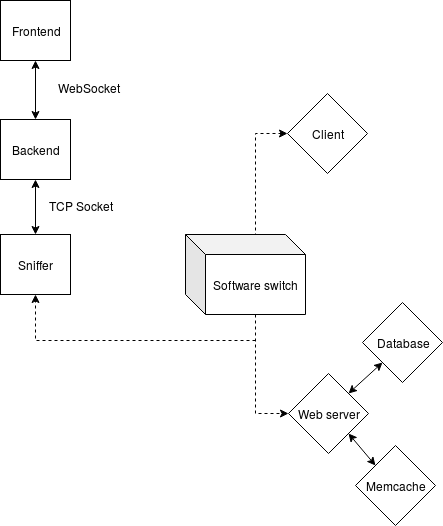
\includegraphics[scale=0.5]{assets/app-architecture.png} \\
	\textbf{Figure 1.1.1 - Monitoring Application integration
	in a Cloud system}
	\end{center}

	\subsection{Server access and source file location}
	\subsubsection{Frontend}

    To access the hosted frontend component:
    \begin{verbatim}
ssh username@bmj-cluster.cs.mcgill.ca
ssh node-02
cd /home/lfesse/monitoring_tool/nodejs-frontend
\end{verbatim}

    The Express server listens for http requests on the 3000 port.
    To reach the frontend server from an external server, use the following address: \\ 
	\url{http://bmj-cluster.cs.mcgill.ca:12230/}
	
\subsubsection{Backend}
To access the hosted backend component (Docker container):
\begin{verbatim}
ssh username@bmj-cluster.cs.mcgill.ca
ssh compute-04
sudo docker exec -it rust_backend bash
cd /home/lfesse/www/rust-backend
\end{verbatim}

    The backend program opens a websocket connection listenning on the 80 port
    To send an incomming request to the websocket from an external server, use the following address: http://bmj-cluster.cs.mcgill.ca:15480/

\subsubsection{Sniffer}
To access the hosted sniffer component: 
    \begin{verbatim}
ssh username@bmj-cluster.cs.mcgill.ca
ssh compute-04
cd /home/lfesse/www/monitoring_tool/c-http-sniffer 	
\end{verbatim}

   
    The sniffer program opens a tcp connection listenning on the 3000 port
    To send an incomming request to the socket from an external server, use the following address: http://bmj-cluster.cs.mcgill.ca:15430/

\subsection{Local development}

After proceeding to the local installation of each component (see section 2.2, 3.1, 4.1 and 5.1), you can locally run the application with the following procedure:
\begin{verbatim}
cd nodejs-frontend/
npm run serve

cd rust-backend/
cargo run

cd c-http-sniffer
scons
./bin/http-sniffer

\end{verbatim}

	
\subsection{Useful commands}
Get a list of all available interfaces to inspect
\begin{verbatim}
ovs-vsctl list interface  
\end{verbatim}

\subsection{Github repository}
	\vspace{-1.5mm}
	All the source code of the project can be find in the following private repository: \\
	https://github.com/laemtl/monitoring\_tool.git

    

\newpage
%%%%%%%%%%%%%%%%%%%%%%%%%%%%%%%%%%%%%%%%%%%%%%%%%%%%%%%%%%%
\section{Frontend}
\vspace{7.5cm}

\textbf{Main dependencies:} Node.js, npm, PM2, Express, Vue, Rickshaw

\vspace{3cm}

The frontend component has two purposes. First, it is the component where an application administrator can indicate what kind of performance monitoring should be performed on their application. 
For that, the frontend provides a form to collect the relevant information (choice of performance metrics, source, destination, analysis duration) (Figure 2.1.1). 
Second, the frontend shows the performance results over time in near real-time (Figure 2.1.2). \\

The frontend part is built on top of Vue.js, a reactive js framework, and Ricksaw.js (Shutterstock), a graphing library using D3.js.

Once an administrator has provided the details of what should be monitored, the frontend sends this information to the backend in json. 
The frontend receives then the performance results for visualization from the backend. 
Communication between frontend and backend is done via a bidirectional and persistent WebSocket (where the frontend is the client initiating the communication and the backend is the server accepting connections). \\

To serve the static frontend files, a simple Express (Node.js) server is used. \\
\\
We also make use of PM2, a production process manager for Node.js applications with a built-in load balancer. 
It allows us to keep our application alive forever, to automatically reload it without downtime if it exits, and to facilitate common system admin tasks.


\subsection{User Interface}

The current UI was built using the Vuetify framework\footnote{https://vuetifyjs.com/en/}. The user can expand a form from the left side, over the ten metric graphs. 
This interface is customizable, each matric can be deselected using the form and the corresponding graph disappears from the screen. \\
\\  
\begin{center}
\frame{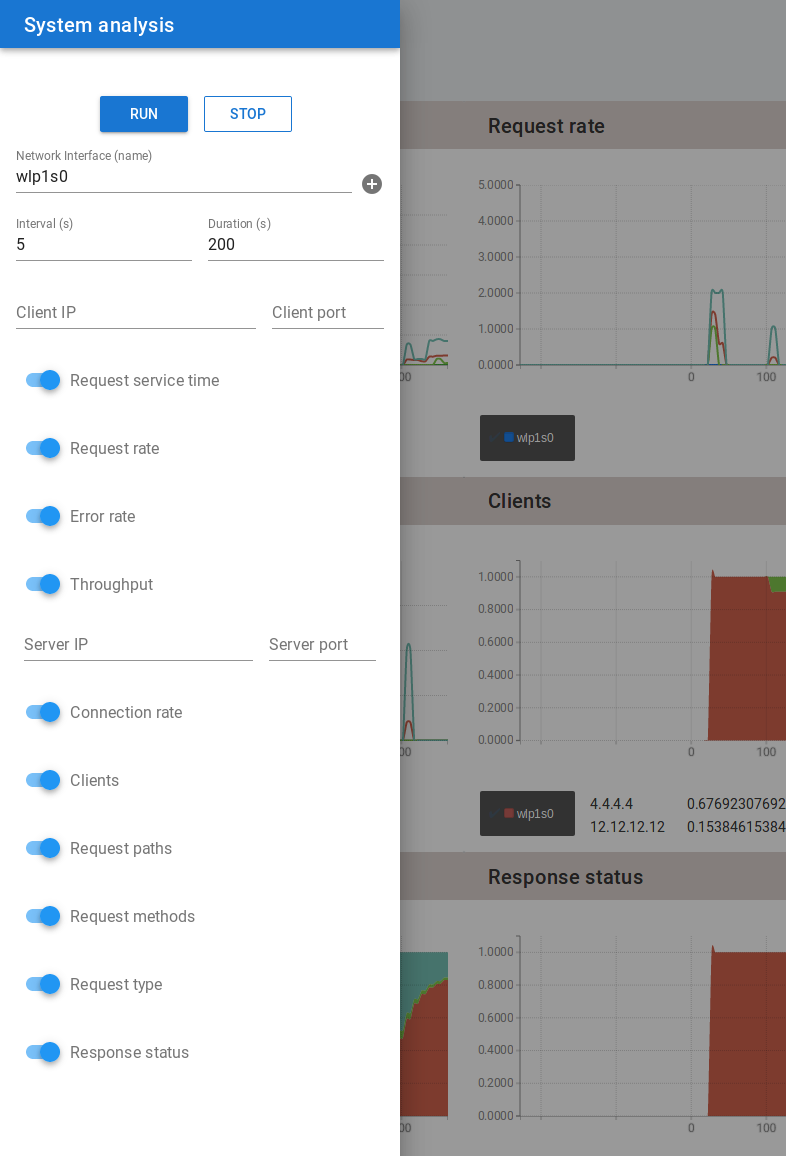
\includegraphics[scale=0.4]{assets/app-form.png}} \\
\textbf{Figure 2.1.1 - Front-End form options}
\end{center}

\begin{center}
	\frame{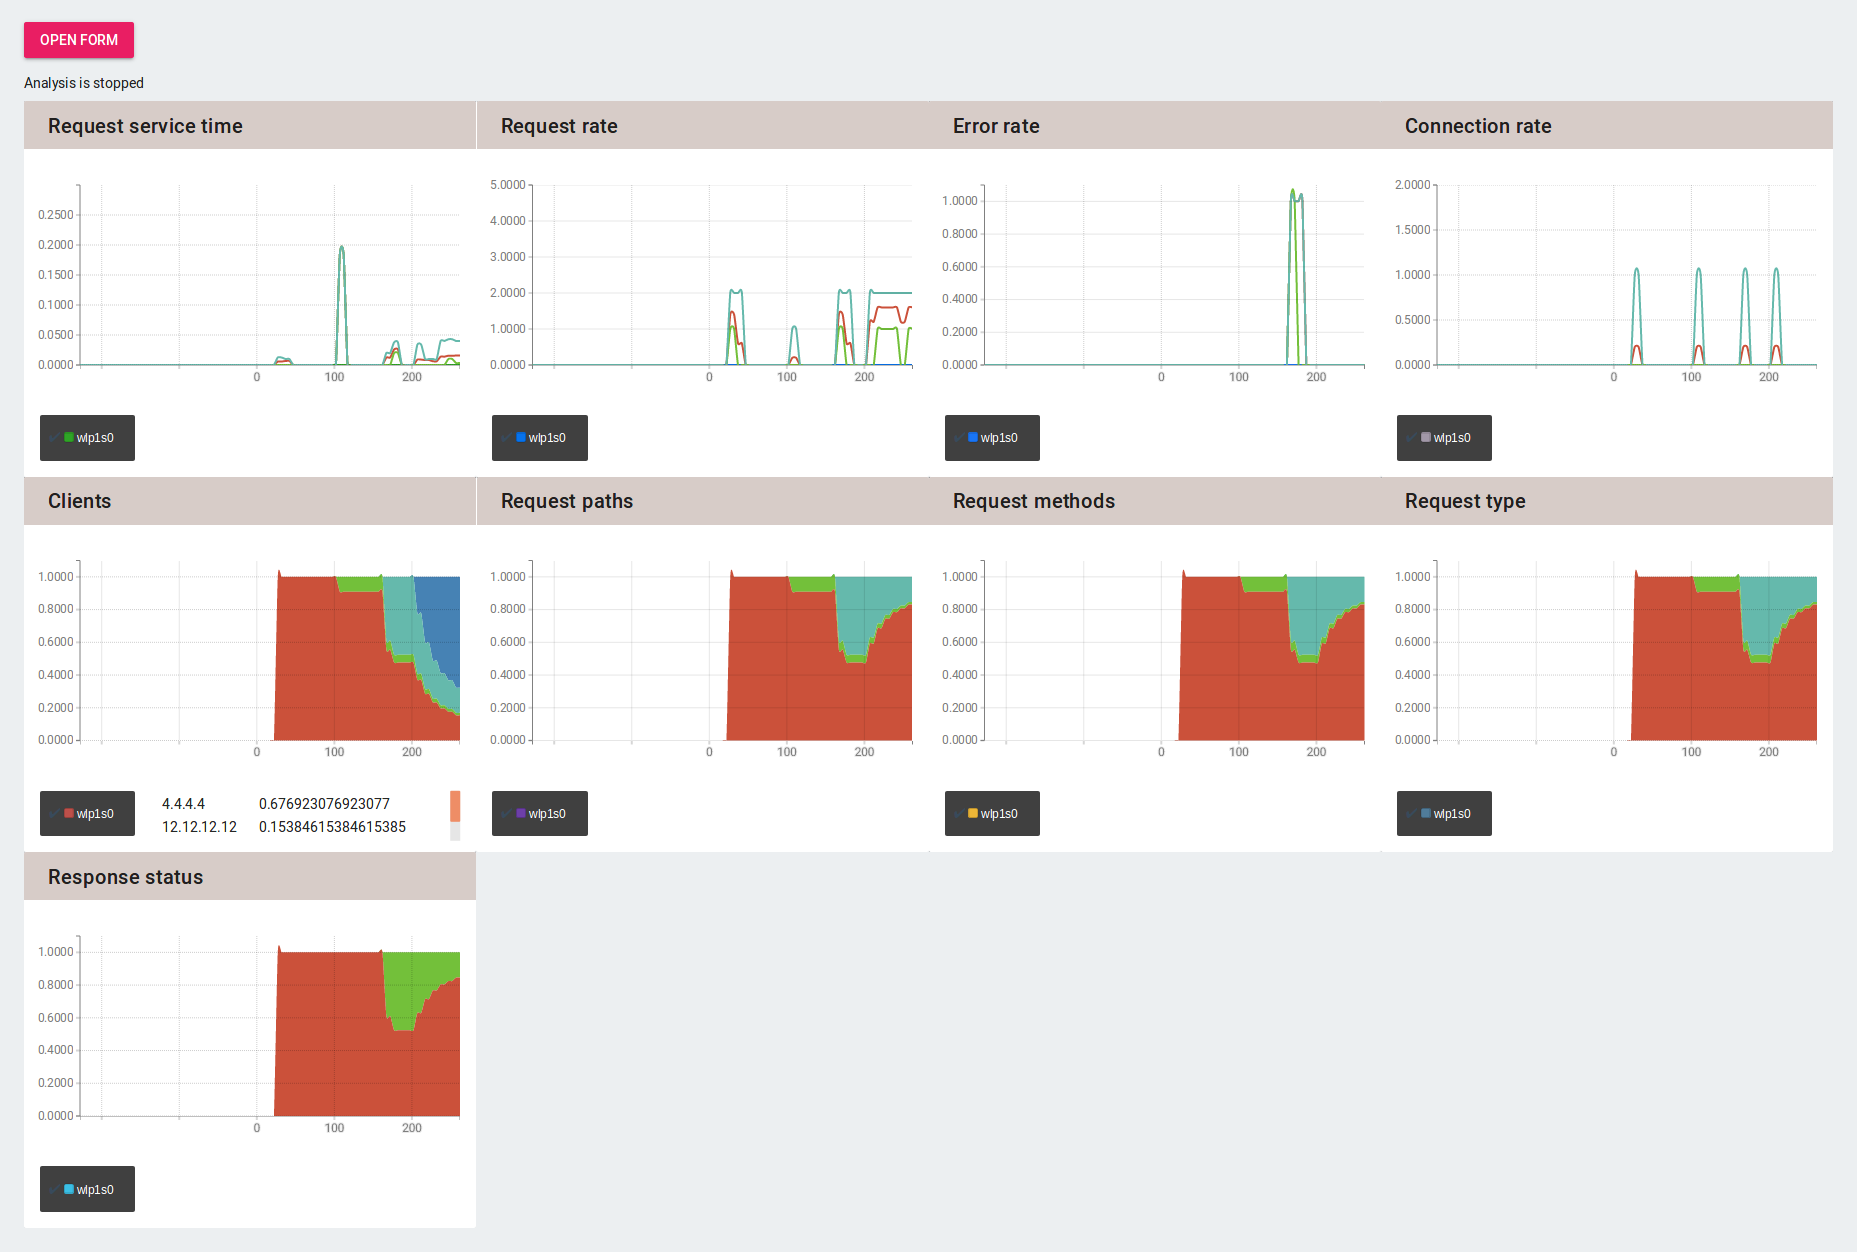
\includegraphics[width=\textwidth]{assets/app-result.png}} \\
	\textbf{Figure 2.2 - Front-End analysis result}
\end{center}


\subsection{Installation} 
\textbf{Install nvm (be sure ~/.bash\_profile exists first)}
\begin{verbatim}
curl -o- https://raw.githubusercontent.com/nvm-sh/nvm/v0.34.0/install.sh | bash
\end{verbatim}

\textbf{Install nodejs 10.8.0}
\begin{verbatim}
nvm install 10.8.0
\end{verbatim}

\textbf{Clone the github repository:}
\begin{verbatim}
git clone https://github.com/laemtl/monitoring_tool.git
\end{verbatim}

\textbf{Install all Node.js dependencies:}
\begin{verbatim}
cd ./monitoring_tools/nodejs-frontend
npm install
\end{verbatim}

\subsection{Usage}
\textbf{Run in dev mode:}
\begin{verbatim}
npm run serve -- --port 3000
\end{verbatim}
Under the dev mode, Express is not needed. \\
\\
\textbf{Build the static files for production:}
\begin{verbatim}
npm run build
\end{verbatim}

\textbf{Start the Express server:}
\begin{verbatim}
node index.js
\end{verbatim}

\subsection{Architecture}
The frontend component lies under /nodejs-frontend. \\

- index.js:
Main file of the Express server.

- node\_modules:
After npm install is invoked, contains all the dependencies of the project.

- dist: 
After a build is invoked, contains all the static files ready fo production.

- src:
Contains all the Vue source files.

	\hspace*{10mm}- App.vue:
	Main template file of the Vue frontend.

	\hspace*{10mm}- main.js:
	Main js file of the Vue frontend.

	\hspace*{10mm}- components/SystemForm.vue:
	Form template file.

	\hspace*{10mm}- components/SystemResultGraph.vue:
	Graph template file.

\newpage
%%%%%%%%%%%%%%%%%%%%%%%%%%%%%%%%%%%%%%%%%%%%%%%%%%%%%%%%%%%
\section{Backend}
\vspace{7.5cm}

\textbf{Main dependencies:} Actix-web, Rust-protobuf 

\vspace{3cm}

The backend, developed in Rust, is mainly a broker between the frontend clients and the sniffers that enables a unified web-based interface for users to the monitoring platform. It forwards the specific monitoring requests from the clients to the relevant sniffer and receives the performance measurement results from the sniffers to be forwarded to the clients. It might also perform some analysis tasks itself should they be too time consuming to be executed at the sniffers that have to work at network traffic speed. \\
\\
Rust is a new compiled language, which is pretty fast (execution time benchmarks show it performs faster than c++) and safer because of a lot of protection mechanisms on compilation time. It also comes with a web server ecosystem which makes it a good choice for a web server. Finally, it can compile in web assembly, which makes it also a good choice to develop frontend features. Apart of the WebSocket connections with the active frontend clients, the backend also maintains a bi-directional TCP socket with each of the sniffers. 
For better performance, the messages sent over TCP are compressed using Google Protocol Buffers.\\
\\
\subsection{Installation} 

\textbf{Install rustup, the Rust installer and version management tool}
\begin{verbatim}
curl https://sh.rustup.rs -sSf | sh
\end{verbatim}

\subsection{Usage} 

\textbf{Run in dev mode:}
\begin{verbatim}
cargo run
\end{verbatim}

\textbf{Build the static files for production:}
\begin{verbatim}
cargo build --release
\end{verbatim}

\textbf{Launch the executable:}
\begin{verbatim}
./target/release/rust-backend
\end{verbatim}

\subsection{Architecture}
The backend component lies under /rust-backend. \\

- build.rs:
Build script, fired at each compilation.

- Cargo.toml:
Configuration file, contains all the dependencies.

- target: 
After a build is invoked, contains all the executable, either for debug or release.

- src:
Contains all the Rust source files.

	\hspace*{10mm}- analysis.rs:
	Handle the Protocol Buffer messages declared in ../analysis.proto.

	\hspace*{10mm}- main.rs:
	Main file of the Rust backend.

\newpage

%%%%%%%%%%%%%%%%%%%%%%%%%%%%%%%%%%%%%%%%%%%%%%%%%%%%%%%%%%%
\section{Protocol Buffer}
\vspace{10.5cm}
For better performance, the messages sent over TCP are compressed using Google Protocol Buffers. In particular, the encoding uses prefix varints which efficienly reduces the size of each transmitted message. 
\subsection{Installation}
All the instructions to proceed to the installation can be found here: \\
https://github.com/protocolbuffers/protobuf/blob/master/src/README.md \\
\\
The sniffer also requires the protobuf-c plugin\footnote{https://github.com/protobuf-c/protobuf-c}. \\
protobuf-c requires a C compiler, a C++ compiler, protobuf, and pkg-config to be installed, along with the autotools (autoconf, automake, libtool).
\begin{verbatim}
git clone https://github.com/protobuf-c/protobuf-c.git
./autogen.sh && ./configure && make && make install
\end{verbatim}

Note that as of version of 1.0.0, the header files generated by the protoc-c compiler contain version guards to prevent incompatibilities due to version skew between the .pb-c.h files generated by protoc-c and the public protobuf-c.h include file supplied by the libprotobuf-c support library. 
Thus, it's a good idea to recompile the .pb-c.c and .pb-c.h files from their source .proto files with protoc-c, rather than shipping potentially stale .pb-c.c and .pb-c.h files that may not be compatible with the libprotobuf-c headers installed on the system in project artifacts like repositories and release tarballs. 

\subsection{Usage}
All the message formats are defined in the file ./analysis.proto. Whenever this file is modified, we need to recompile files which contains data structure definitions and helper functions to support the protocol under C and Rust. \\

\textbf{Compile the c Protobuf files:}
\begin{verbatim}
cd monitoring_tools/
protoc --c_out=. analysis.proto
mv analysis.pb-c.h ./c-http-sniffer/include/analysis.pb-c.h
mv analysis.pb-c.c ./c-http-sniffer/src/analysis.pb-c.c
\end{verbatim}


\textbf{Compile the Rust Protobuf files:}
\begin{verbatim}
cargo run RUST_BACKTRACE=1 
\end{verbatim}

\subsection{Architecture}
The configuration file for all defined messages lies in ./analysis.proto.

\newpage
%%%%%%%%%%%%%%%%%%%%%%%%%%%%%%%%%%%%%%%%%%%%%%%%%%%%%%%%%%%
\section{Sniffer}	
\vspace{7.5cm}

\textbf{Main dependencies:} protobuf-c

\vspace{3cm}

The sniffer is a component that is attached to the software switches of the cloud that route the cloud traffic. The sniffer, written in C, listens to relevant network traffic and performs some of the performance analysis on the fly by analyzing specific network messages.
For doing such analysis work, the sniffer reads and extracts all the information needed from the network packets. The information is then stored in different data structures, typically hashtables (e.g., one for client relevant information, one for paths, etc.). In given time intervals, the individual metrics such as average response times are then computed. On a regular basis, the results are sent to a backend analysis server.
The sniffer requires the network interface name of network flows to be observed, and some analysis configuration (interval, duration, metrics choice). It can run several analysis at the same time.

\subsection{Installation} 
If gcc is already on the system, nothing is needed besides protobuf-c (see section 4.1) and SCons (needs Python):

\begin{verbatim}
pip install scons
\end{verbatim}

\subsection{Architecture}
The sniffer has the capability to run under 3 modes: \\
    - offline; \\
    - live standalone; \\
    - live server; \\

The sniffer was heavily modified for the current implementation, and offline functionality has not has been tested yet. 
There may be some adjustments needed in order to make it work properly. \\
\\
Amongst the improvements made, we reduced the latency between each packet capture, minimizing the risk of packet drop, by delaying the packet processing and filtering process.
Instead, the thread handling the capture save each packet in a queue and let another thread doing the filtering/processing task. \\
\\
The live standalone mode may benefit from some additional flags in order to offer the same functionalities as the interface/server mode as a future improvement. \\
\\
Under the server mode, a thread opens a TCP connection, listenning for incoming request. \\
\\
The program uses 7 other threads for each analysis routine: \\
- job\_pkt: process the raw packets queue, discarding non HTTP packets ; \\
- job\_pkt\_q: process the queue of filtered HTTP packets, converting them to flows ; \\
- job\_flow\_q: process the flows which have received their last packet (connection closed) ; \\
- job\_scrb\_htbl: clean all the remaining flows ; \\
- timer: manage the interval and duration timers ; \\
- capture: capture all the packets on the given interface placing them in a raw\_pkt\ queue. \\
\\
Each of these threads shares common variables. 
The Data struct (see data.h) stores all these common variables. When a new analysis is spawned, a block of memory is allocated to store a Data block, and its pointer is stored in a pthread\_key\_t, a thread-specific variable.
This strategy allows us to read/write elements of these common variables from anywhere within theses 4 threads functions. It act as a thread safe global variable.
    
%%%%%%%%%%%%%%%%%%%%%%%%%%%%%%%%%%%
% ------- Code & Examples ------- %
%%%%%%%%%%%%%%%%%%%%%%%%%%%%%%%%%%%
\vspace{1cm}	
\begin{DashedDefinition}{}
[The pthread\_key\_create() function shall create a thread-specific data key visible to all threads in the process. 
Key values provided by pthread\_key\_create() are opaque objects used to locate thread-specific data. 
Although the same key value may be used by different threads, the values bound to the key by pthread\_setspecific() are maintained on a per-thread basis and persist for the life of the calling thread.
\footnote[0]{\url{https://linux.die.net/man/3/pthread_key_create}}
\end{DashedDefinition}

\vspace*{0.75\baselineskip}
%===============================

The sniffer component lies under /c-http-sniffer. \\
\\
- SConscript: Compilation configuration file. \\
- protobuf-c.c: protobuf-c library. \\
- analysis.pb-c.c: File generated by protobuf-c. \\
- client.c, conn.c, req\_path.c, req\_type.c, rsp\_status.c: Metrics computation. \\
- data.c: Flows and pairs processing, metrics computation.\\
- flow.c \\
- flow\_hash\_table.c \\
- flow\_queue.c \\
- hash\_table.c \\
- http.c \\
- main.c: Main file of the sniffer program. Detect the mode and spawn the major threads. \\
- order.c \\
- packet.c: Packet library. \\
- packet\_queue.c \\
- queue.c: Queue library. \\
- raw\_pkt\_queue.c \\
- server.c: Server functionalities. \\
- tcp.c \\
- timer.c \\
- util.c: Helper functions.

\subsection{Usage}
./ycsb run jdbc
-P ../workloads/workloadc
-p jdbc.driver=com.mysql.jdbc.Driver
-p db.url=jdbc:mysql://172.16.1.8:3306/YCSB
-p db.user=root
-p db.passwd=root
-s
-threads 20
-target 0
-p measurementtype=timeseries
-p timeseries.granularity=20000

To compile and execute the program: \\
cd c-http-sniffer/ \\
scons \\

Run in Standalone mode:
./bin/http-sniffer -i interface

Run in Server mode:
./bin/http-sniffer



\newpage
%%%%%%%%%%%%%%%%%%%%%%%%%%%%%%%%%%%%%%%%%%%%%%%%%%%%%%%%%%%
\section{Traffic generators}	
\vspace{10.5cm}	
Traffic can be simulated with the following two tools: YCSB, a modified benchmark tool and ScapyTrafficGenerator, a network traffic simulator to test our system.

	\subsection{YCSB}
	
	YCSB is originally a database benchmark where a YCSB client sends requests to a database. Our extended version has added a Tomcat webserver as frontend for the client (which was modified to communicate with the Tomcat server); the Tomcat server has access to a MySQL database and a Memcache server. Each component is deployed in a separate container and all containers are connected by an OVS switch configured via Openflow. The clients submit a predefined workload of HTTP requests to the web server whereby each request retrieves data from either the database or the memory cache. Recent results are cached in the Memcache server. The data-base schema and the query requests follow the YCSB benchmark. \\
\\
\textbf{Log on the docker container hosting YCSB:}
\begin{verbatim}
ssh username@bmj-cluster.cs.mcgill.ca
ssh compute-04
sudo docker exec -it ycsbclient_nano /bin/bash
\end{verbatim}

\pagebreak


\textbf{Configure the traffic simulation duration:}
\begin{verbatim}
nano YCSBCLIENT/workloads/workloadc
# Edit the following value (in sec): maxexecutiontime=20
\end{verbatim}
	
\textbf{Start YCSB:}
\begin{verbatim}
cd YCSBCLIENT/bin/
./ycsb run jdbc 
-P ../workloads/workloadc 
-p jdbc.driver=com.mysql.jdbc.Driver
-p db.url=jdbc:mysql://172.16.1.8:3306/YCSB 
-p db.user=root 
-p db.passwd=root 
-s 
-threads 20 
-target 0 
-p measurementtype=timeseries 
-p timeseries.granularity=20000
\end{verbatim}
   	\subsection{ScappyTrafficGenerator}\label{subsec:mathenvironments}
The relevant documentation can be found here: https://pypi.org/project/ScapyTrafficGenerator/ \\
\\
\textbf{Start ScappyTG:} 
\begin{verbatim}
ScapyTrafficGenerator -X http -r '-X 1 -F /test.txt 
-i interface -s 2.2.2.2 -S 20 -d 5.5.5.5 -D 80 -T 10 -x 200 -u /path/url'
\end{verbatim}
\newpage
%%%%%%%%%%%%%%%%%%%%%%%%%%%%%%%%%%%%%%%%%%%%%%%
\end{document}